% !TEX root = main.tex

\section{Path explosion}

One of the main challenges of symbolic execution is the path explosion problem. Since symbolic execution may fork off a new interpreter at every branch, the total number of interpreters may be exponential in the number of branches of the program. This impact both time and space, as a symbolic executor may need to keep track of an exponential number of pending branches to be explore. A common approach is to compute an under-approximation of the analysis that only explores a relevant subset of the state space.

% ---------------------------------------------------------------------------------------------------
\subsection{Pruning unrealizable paths}

A common technique for reducing the path space is invoking the constraint solver at each branch, pruning branches that are not realizable. 

From warm-up example\mynote{IF: I removed from the warm up the non-forking case. Must be explained here}:

The evaluation of a conditional branch ${\tt if}~e~{\tt then}~s_{true}~{\tt else}~s_{false}$ affects the path constraint. Two scenarios are possible:
    \begin{enumerate}
      \item {\em Non-forking}: if $e$ is evaluated as always true (resp., false) under the assumptions in the current state, the proper branch is taken and the symbolic execution advances to $s_{true}$ (resp., $s_{false}$);
      \item {\em Forking}: if $e$ cannot be evaluated without instantiating values for one or more of its symbols, the symbolic execution is forked by creating two execution states with path constraints $pct_{true}$ and $pct_{false}$, respectively, corresponding to the two {\tt if} branches. Namely, $pct_{true}=pct \wedge e_s$ and $pct_{false}=pct \wedge \neg e_s$, where $e_s$ is a symbolic expression obtained by evaluating $e$. 
%        \[ (s_{true}, pc_{true}) \text{ where } pc_{true} = pc \wedge e \]
%        \[ (s_{false}, pc_{false}) \text{ where } pc_{false} = pc \wedge \neg e \]
    Symbolic execution proceeds on both states in parallel.
    \end{enumerate}


\begin{figure}[t]
  \centering
  \begin{adjustbox}{width=1\columnwidth}
  \begin{small}
  \begin{tabular}{| l || l || l |}
    \hline      
    Heuristic & Goal & Discussed by \\ \hline\hline
    BFS & maximize coverage & \cite{CKC-TOCS12,PEX-TAP08} \\
    DFS & exhaust paths, minimize memory usage & \cite{EXE-CCS06,CKC-TOCS12,PEX-TAP08,DART-PLDI05} \\
    random path selection & randomly pick a path with probability based on its length & \cite{KLEE-OSDI08} \\
    %low-covered code & prioritize paths that execute low-covered code  & \cite{EXE-CCS06} \\
    code coverage search & prioritize paths that may explore unexplored code & \cite{EXE-CCS06,KLEE-OSDI08,MAYHEM-SP12,CKC-TOCS12,GV-ISSTA02} \\
    buggy-path-first & prioritize bug-friendly path  & \cite{AEG-NDSS11} \\
    loop exhaustion & fully explore specific loops  & \cite{AEG-NDSS11} \\
    symbolic instruction pointers & prioritize paths with symbolic instruction pointers & \cite{MAYHEM-SP12} \\
    symbolic memory accesses & prioritize paths with symbolic memory accesses & \cite{MAYHEM-SP12} \\ 
    fitness function & prioritize paths based on a fitness function & \cite{XTD-DSN09,CS-CACM13,XTD-DSN09} \\
    kill path & filter uninteresting path & \cite{CKC-TOCS12} \\
    
    \hline  
  \end{tabular}
  \end{small}
  \end{adjustbox}
  \caption{List of path selection heuristics.}
  \label{tab:heuristics}
\end{figure}


% ---------------------------------------------------------------------------------------------------
\subsection{Bounding computational resources}
\label{heuristics}

Another common approach is to limit the amount of resources symbolic execution is allowed to use. For instance, the computation may time out after a certain amount of time. Since only a fraction of paths may be explored, the search should be prioritized by looking at the most promising paths first. There are several strategies for selecting or generating the next path to be explored. We now briefly overview some of the most interesting techniques that have been shown to be effective in prior works.

\subsubsection{Search heuristics}

Given a set of unexplored paths, a search heuristics should select the most promising path to explore. Many prior works have introduced novel search strategies, showing their effectiveness in specific application contexts. These heuristics have often been tailored for helping the symbolic engine to achieve a specific goal (e.g., overflow detection). Finding a universally optimal strategy for prioritizing path exploration remains an open problem. Table~\ref{tab:heuristics} provides a sample of the most interesting search heuristics discussed in prior works. 

The most common strategies are {\em depth-first search} and {\em breadth-first strategy}. The former continuously expands a path as much as possible, before backtracking to the last unexplored branch. The latter explores all unexplored path in parallel, repeatedly expanding each of them of a fixed slice. DFS is often adopted for minimizing the memory usage of the symbolic engine: since the chosen path will be sooner or later fully explored, the memory needed for keeping its state will be released as well. Unfortunately, paths containing loops and recursion can easily stall the symbolic engine. For this reason, some tools prefer to perform path prioritization using BFS. Although the memory pressure can be higher, this strategy may allow an engine to quickly explore diverse paths and possibly detecting interesting behaviors. On the other hand, if the ultimate goal requires to fully explore a set of paths, BFS may take a very long time.

Another very popular strategy is {\em random path selection} that, as its name would suggest, randomly picks a path for exploration. This kind of heuristic has been refined in several variants. For instance,~\cite{KLEE-OSDI08} assigns probabilities to paths based on their length and based on the branch arity. In other words, it favors paths that have been explored for fewer times, preventing starvation given by loops and other path explosion causes.

Several works~\cite{EXE-CCS06,KLEE-OSDI08,MAYHEM-SP12,CKC-TOCS12} have instead presented heuristics aimed at maximizing the code coverage. For instance, the {\em coverage optimize search} discussed in~\cite{KLEE-OSDI08} computes a weight for each state and then randomly selects a state according to these weights. The weight is obtained by taking into account the minimum distance to an uncovered instruction, the call stack of the state, and whether the state recently covered new code.

Other search heuristics try to prioritize paths that may likely reach an interesting state. For instance, the {\em buggy-path first} strategy in~\cite{AEG-NDSS11} picks paths whose past states have contained small but unexploitable bugs. Indeed, if a path contains some small errors then it is likely that it has not been properly tested. As a consequence, there is a good chance that future states may contain some interesting, and hopefully exploitable, bugs. Similarly, the {\em loop exhaustion} strategy~\cite{AEG-NDSS11} explores paths that are visiting loops. This approach is inspired by the practical observation that common programming mistakes in loops may lead to buffer overflows or to other memory related errors. \cite{MAYHEM-SP12} instead gives priority to paths where symbolic memory accesses are identified or to paths where symbolic instruction pointers are detected. 

Fitness functions have been extensively used in the context of search-based test generation~\cite{M-STVR04}. A fitness function measures how close an explored path is in achieving test target coverage. Several papers~\cite{XTD-DSN09,CS-CACM13,XTD-DSN09} have applied this idea in the context of symbolic execution. As an example,~\cite{XTD-DSN09} introduced {\em fitnex}, a strategy for concolic execution that prioritize paths that are {\em closer} to take a specific branch. In more detail, given a branch condition of the form $|a - c| == 0$ and a path that has reached the branch, fitnex computes a closeness equal to $|a - c|$. Similar fitness values can be computed for other kinds of branch conditions. The path with the lower fitness value for a branch is selected by the symbolic engine. Paths that have not yet reached the branch, get the worst-case fitness value.

\begin{comment}
\begin{itemize}

  \item \cite{AEG-NDSS11}:
  \begin{itemize}
    \item {\em buggy-path-first}: priority to path that shown to contain errors (even if not exploitable)
    \item {\em loop exhaustion}: give priority to path that are exhausting a loop. In practice this can hit exploitable bugs (buffer overflows), but can prevent progress. Allow only one executor that is exhausting a loop, perform aggressive preconditioned symbolic execution.
  \end{itemize}

  \item {\em less covered code}: \cite{EXE-CCS06} uses a mixture of best-first and depth-first search. Best-first approach uses heuristic that give high priority to the path which is blocked at the line that has been executed the fewest number of times. The picked path is executed with DFS for a limited amount of time in order to avoid starvation. 

  \item \cite{KLEE-OSDI08} interleaves in a round robin fashion these strategies:
  \begin{itemize}
    \item {\em random path selection}: build a binary tree structure of all the state (each state is always created due to a fork from a parent). Assign same probability of being executed among states of the same subtree. Avoid starvation by given priority to states high in the tree.
    \item {\em coverage optimize search}: assign weights based on how much new code has been covered by a path. Pick up state randomly using weights as probability.
  \end{itemize}
  Each state is executed only for a time slice defined both as maximum number of instructions and as maximum amount of time.

  \item \cite{SAGE-NDSS08}:

  \item \cite{MAYHEM-SP12} same heuristics as~\cite{SAGE-NDSS08} and~\cite{KLEE-OSDI08}:
  \begin{itemize}
    \item executors exploring new code have high priority
    \item executors that identify symbolic memory accesses have high priority
    \item executors where symbolic instruction pointers are detected have high priority
  \end{itemize}

  \item \cite{CS-CACM13} mentions that a {\em fitness function} can be used to drive exploration of input space. Some examples: \cite{BHH-ASE11,LMH-JSS10}.

  \item Priority-based selection in~\cite{CKC-TOCS12}:
    \begin{itemize}
      \item bread-first search
      \item depth-first search
      \item max coverage heuristic
      \item path killer heuristic: kill paths that are no longer of interest (e.g., kill path that repeats sequence of program counters more than $n$ times)
    \end{itemize}

\end{itemize}
\end{comment}

\subsubsection{Dynamic Test Generation}
%\subsubsection{Generational Search}
%{\em Use concolic execution to generate useful (random) inputs.} 
Starts concrete execution using a random (concrete) input and for each taken branch tracks the input constraints by observing the branch condition. When the execution is completed, restart another concrete execution using a different concrete random input that is compliant with the constraints but explore a new path. It is sufficient to negate a single constraint given by a conditional branch, to explore a different path. Keep track of taken branches with binary values. An algorithm for maximizing coverage is proposed in~\cite{DART-PLDI05}. Notice that the symbolic execution is performed in parallel with the concrete execution. Related examples are~\cite{SAGE-NDSS08,DRILLER-NDSS16}. \mynote{Add paper on hybrid concolic testing}In particular,~\cite{DRILLER-NDSS16} is an example of {\em symbolic-assisted fuzzing}: their technique temporarily exploits concolic execution only when a fuzzer cannot generate a valid input to explore an uncovered branch.

\paragraph{An example}\mynote{Improve this discussion} Given a concrete input, an application will execute only a subsets of its basic blocks $B_i$. Moreover, they will be executed following a specific order. For instance, the program execution shown in Figure~\ref{fig:example-concrete-execution}a has executed the sequence of basic blocks $\{B_1, B_2, B_4, B_6\}$. Other blocks, such as $B_3$, have not been executed due to non-taken branches. Driven by the concrete execution, a symbolic execution engine may trace symbolic constraints on the taken branches and then generate an input that forces the execution to take a never-taken branch. For instance, if the symbolic execution engine may want to generate an input that executes basic block $B_5$, then it traces the constraints on the two taken branches and then negate the constraint on the branch that leads the execution toward $B_5$. Figure~\ref{fig:example-concrete-execution}b provides the logical steps performed by the engine.

\begin{figure}[t]
  \vspace{-3mm}
  \centering
  \begin{subfigure}{.5\textwidth}
    \centering
    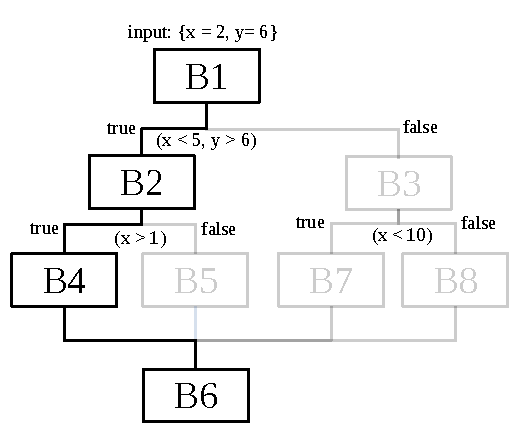
\includegraphics[width=0.9\columnwidth]{images/concrete-execution} 
    %\label{fig:sub1}
    \vspace{15mm}
    \caption{}
  \end{subfigure}%
  \begin{subfigure}{.5\textwidth}
    \centering
    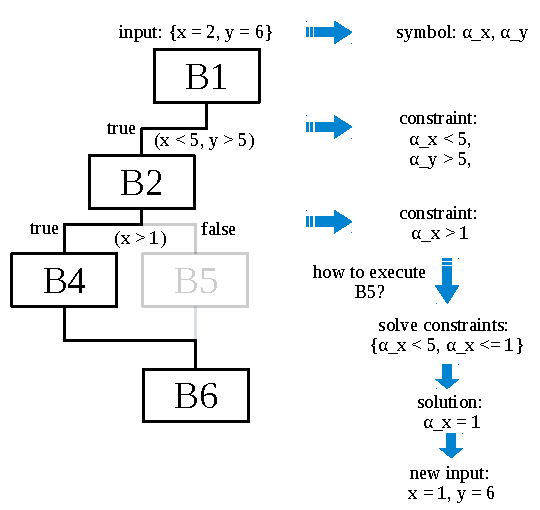
\includegraphics[width=1.0\columnwidth]{images/concolic-execution} 
    %\label{fig:sub2}
    \caption{}
  \end{subfigure}
  \caption{(a) a concrete execution of a program. Only a subset of basic blocks is executed. The sequence of executed basic blocks is $\{B_1, B_2, B_4, B_6\}$. (b) concolic execution for generating an input that executes $B_5$.}
  \label{fig:example-concrete-execution}
  \vspace{-3mm}
\end{figure}

% ---------------------------------------------------------------------------------------------------
\subsection{Preconditioned symbolic execution}
\label{precontioned-symbolic-execution}

\cite{AEG-NDSS11} has proposed {\em preconditional symbolic execution} as a novel method to target symbolic execution towards certain subsets of the input state space. The state space subset is determined by the precondition predicate $\Pi_{prec}$: inputs that do not satisfy $\Pi_{prec}$ will not be explored. The intuition for preconditioned symbolic execution is that we can narrow down the state space we are exploring by specifying exploitability conditions as a precondition, e.g., all symbolic inputs should have the maximum size to trigger buffer overflow bugs. The main benefit from preconditioned symbolic execution is simple: by limiting the size of the input state space before symbolic execution begins, we can prune program paths and therefore explore the target program more efficiently.
Note that preconditions cannot be selected at random. If a precondition is too specific, we will detect no bugs or exploits; if it is too general, we will have to explore almost the entire state space. %Thus, preconditions have to describe common characteristics among exploits (to capture as many as possible) and at the same time it should eliminate a significant portion of non-exploitable inputs.\\

Preconditioned symbolic execution enforces the precondition by adding the precondition constraints to the path predicate during initialization. Adding constraints may seem strange since there are more checks to perform at branch points during symbolic execution. However, the shrinking of the state space -- imposed by the precondition constraints -- outweighs the decision procedure overhead at branching points. When the precondition for a branch is unsatisfiable, we do no further checks and do not fork off an interpreter at all for the branch.% We note that while we focus only on exploitable paths, the overall technique is more generally applicable.\\

\paragraph{Preconditions} Kinds of preconditions:
\begin{itemize}
\item {\em None}. There is no precondition and the state space is explored as normal.
\item {\em Known Length}. The precondition is that inputs are of known maximum length, e.g., a network packet has a fixed size.
%Static analysis techniques can be used to automatically determine this precondition.
\item {\em Known Prefix}. The precondition is that the symbolic inputs have a known prefix, e.g., a fixed header string such as the initial {\em magic code} of a binary input file, or a network packet header.
\item {\em Fully Known}. 
%Concolic execution [24] can be viewed as a specific form of preconditioned symbolic execution where the precondition is specified by 
 %a single program path as realized by 
%a concrete example input. For instance, we may already have an input that crashes the program, and we use it as a precondition to determine if the executed path is exploitable. %See Section~\ref{concolic-execution} for a more detailed discussion of this technique.
\end{itemize}

\paragraph{An example} Consider the example\mynote{citation to example source, if any?}:

\begin{figure}[t]
\begin{small}
\begin{lstlisting}[basicstyle=\ttfamily\small]
    // N symbolic branches 
    if (input[0] < 42) [...]
    [...]
    if (input[N - 1] < 42) [...]

    // symbolic loop
    strcpy(dest, input); 

    // M symbolic branches
    if (input[N + 1] < 42) [...]
    [...]
    if (input[N + M - 1] < 42) [...]
\end{lstlisting}
\end{small}
\caption{State space size.}
\label{fig:state-space-size}
\end{figure}

where {\tt input} is an array of $S\ge N+M$ bytes. Impact of preconditions:
\begin{itemize}
  \item {\em None}. No constraint is added. State space size is $2^N \cdot S \cdot 2^M$.
  \item {\em Known Length}. For instance, we add constraint that $(S - 1)$ bytes of {\tt input} are not equal to \textbackslash0. Since the symbolic loop is known, then the state space size is reduced to $2^N \cdot 2^M$.
  \item {\em Known Prefix}. For instance, we add constraint that the $P$ bytes of {\tt input} are known ($P < N < S$). Since first $P$ branches and first $P$ iterations are concrete, then state space is $S \cdot 2^{N-P} \cdot 2^M$.
  \item {\em Concolic Execution}. We decide the exact values for all bytes of {\tt input}. The state space size is $1$.
\end{itemize}

%\subsection{Dynamic symbolic execution}

%Dynamic symbolic execution refers to a body of techniques that exploit execution with concrete values to explore [...].

% ---------------------------------------------------------------------------------------------------
\subsection{Under-constrained symbolic execution} 
\label{under-constrinained}

By isolating a function from the rest of the program, we can perform symbolic execution on it. The results from this analysis can be exploited when any other program is symbolically executed and a call to the function is present. However, detected errors in the isolated function may be false positives since some of the input values may never been valid when the function is actually executed in the context of the full program. Some prior works (e.g., \cite{CS-ICSE05}\mynote{check this paper}) first analyze code in isolation and then test the generated crashing inputs using concrete executions. 

{\em Under-constrained symbolic execution}~\cite{ED-ISSTA07} is a technique that performs symbolic execution of an isolated function but clearly marks which symbols are {\em under-constrained} to distinguish them from the {\em exactly-constrained} symbols.

Errors due to concrete values and exactly-constrained symbols are treated as true positives. On the other end, errors due to under-constrained are treated as true positives only if {\em all} solutions to the currently known constraints on the symbols cause the error to occur. Otherwise the negation of the error is added to the constraint set and the symbolic execution of the isolated function is continued. In other words, an error is reported if and only if it is {\em context-insensitive}. Notice that a symbol may initially be under-constrained and then become exactly constrained. For instance, consider the following piece of code:

    \begin{lstlisting}[basicstyle=\ttfamily\small]
    assert(a != 0); // no knowledge about this variable
    a = 0;          // from now on we know the value of a
    assert(a != 0); // we always hit this error: context-insensitive! 
    \end{lstlisting}

If {\tt a} is marked as under-constrained, then the first {\tt assert} will not trigger an error: indeed, there is at least one possible value for the symbol associated to {\tt a} that does not hit the error. Conversely, the second {\tt assert} will always trigger an error since {\tt a} has a concrete value and it's not anymore under-constrained.\\

Although this technique is not able to find {\em all} the possible errors in a function, it still can find interesting bugs. Moreover, since symbolically executing a full program may be unfeasible, this technique can make it feasible to test tons of line of code in a reasonable amount of time. In particular, this technique allows an engine to skip code: if a function or any other construct (e.g., a loop) may be troublesome for symbolic execution, it can be skipped by just marking the locations affected by it as under-constrained. However, a possible implementation issue is given by the propagation of under-constrained symbols: given the line of code {\tt if (s < t)}, if {\tt t} is under-constrained while {\tt s} is exactly constrained then when the symbolic execution is proceeded into the two possible branches, {\tt s} must be marked as under-constrained. Some optimization may be needed in order to minimize this propagation effect.

\begin{comment}
\paragraph{Under-constrained KLEE}\mynote{I will revise this (emilio)} In~\cite{UCKLEE-USEC15}, KLEE~\cite{KLEE-OSDI08} has been extended in order to support under-constrained symbolic execution . In particular, these are some of the main improvements:
\begin{itemize}
  \item {\em Lazy initialization.} Whenever there is a pointer that is not concrete and without any active constraint (i.e., it is unbound), its value is checked against {\tt NULL} then two path are analyzed: (a) where the pointer is {\tt NULL} and (b) where the pointer is pointing to a freshly allocated block of memory, whose content is marked as unbound.This means that pointer aliasing is assumed to not occur. In both paths, the pointer is not longer unbound.  In path (b), any test against the pointer is known and dereferences will be successfully resolved. Lazy initialization is common for data structure and thus it is common to bound its maximum length (i.e., {\em k-bounding}) in order to prevent the engine from allocating an unbounded number of objects.
  \item {\em Patch checking.} The main goal of~\cite{UCKLEE-USEC15} is to detect if a patch has introduced new bugs. In order to do so, it symbolically executes two compiled versions of a function: $P$, the unpatched version, and $P'$, the patched version. If it finds any execution paths along which $P'$ crashes but $P$ does not (when given the samce symbolic inputs), it reports a potential bug. Indeed, due to missing input preconditions, not all crashes are real bugs: if both $P$ and $P'$ crash on an input, then maybe the crash is given by the unknown preconditions. 
  \item {\em Pruning techniques.} Using a static cross-checker (that navigates the control-flow graph and marks differing basic block between $P$ and $P'$), \cite{UCKLEE-USEC15} prunes paths that have never executed a differing basic block and that cannot reach a differing basic block from their current program counter and call stack. Moreover, $P'$ is executed before executing $P$, allowing the system to prune paths that return from $P'$ without triggering an error, or that trigger an error without reaching different blocks.
  \item {Dealing with false positives.} Two approaches are pursued to limit false positives:
    \begin{itemize}
      \item {\em manual annotations}: examples are data types invariants or preconditions upon function calls.
      \item {\em automated heuristics}: {\em must-fail} heuristics identify errors that must occur for all input values following that execution path. For instance, {\em belief-fail} heuristic checks if a function contradicts itself (e.g., a code checks that a pointer is {\tt NULL} and then dereferences it). Another variation of must-fail heuristic is {\em concrete-fail} that an assertion failure or memory errors was triggered by a concrete condition or pointer.
    \end{itemize}
  \item {\em Rule-based checkers.} Several rule-based checkers have been built on top of UCKLEE. They do a similar job such as other dynamic tools (e.g., {\em memcheck} for memory leaks and uninitialized data) but reasoning on all possible paths, not just the concrete ones. Moreover, user inputs can be considered as fully constrained (i.e., no assumption is valid on it since the code should sanitize it). 
  \item {\em Optimizations.} Some optimizations:
    \begin{itemize}
      \item Symbolic objects have a symbolic size: whenever there is an access to the object content, the system verifies if the offset could exceed the object's symbolic size. whenever path is considered where the offset does not exceed the symbolic size, then a lower bound on the symbolic size is set.
      \item Some library functions (e.g., {\tt strlen}) have been replaced with variants that do not lead to path explosion
      \item Scores of rules to simplify symbolic expressions
      \item {\em lazy constraints}: defer evaluation of constraints using a solver as much as possible. For instance, if there is an hard constraint on branch, take both branches and if an error is found check if that branch was actually valid.
      \item function pointers should be made concrete by the user.
    \end{itemize}

\end{itemize}
\end{comment}

% ---------------------------------------------------------------------------------------------------
\subsection{State merging}

Several static program analysis techniques such as abstract interpretation merge states corresponding to different paths into a state that over-approximates them. In a precise symbolic execution, however, merging is not allowed to introduce any approximation or abstraction, and therefore can only change formulas to have them characterize sets of execution paths. In other words, a merged state will be described by a formula that represents the disjunction of the formulas that would described the individual states if they were kept separate.

\paragraph{An example} Let's consider the following piece of code (taken from~\cite{VERITESTING-ICSE14}):\mynote{customize example and improve discussion}
    \begin{lstlisting}[basicstyle=\ttfamily\small]
    B1: if (x > 1) 
    B2:   y = 42;
    B3: else if (x < 42) 
    B4:    y = 17;
    B5: else ;
    B6: ;
    \end{lstlisting}
Then a symbolic execution engine may perform state merging in the following way:
\begin{figure}[H]
  \centering
  \vspace{-3mm}
  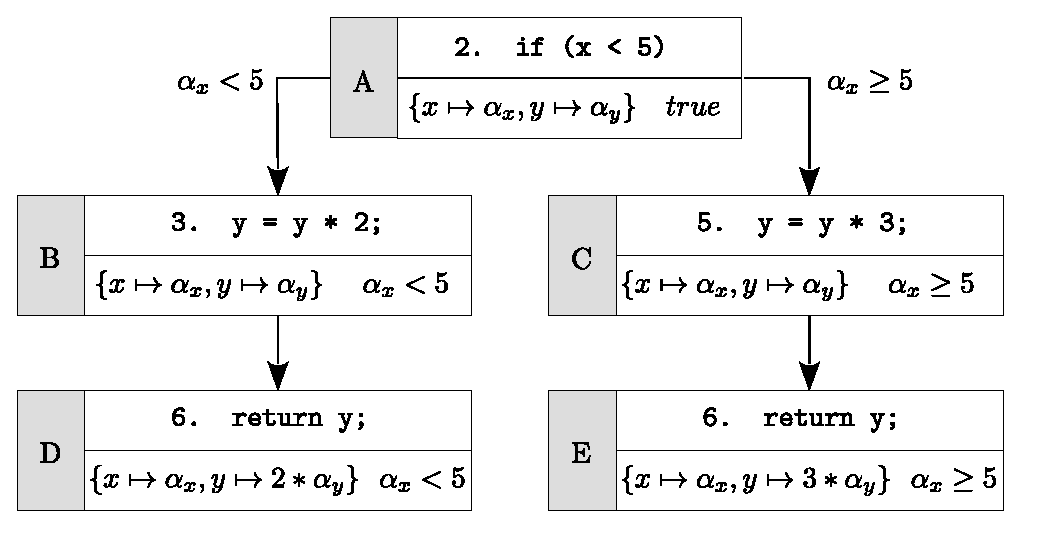
\includegraphics[width=0.65\columnwidth]{images/state-merging} 
  \vspace{-3mm}
  %\label{fig:example-symbolic-execution}
\end{figure}
where {\em ite} statements represents {\tt if-then-else} statements and $\bot$ stands for a non-taken branch.

\paragraph{Trade-off} Early work~\cite{G-POPL07,HSS-RV09} has shown that merging techniques effectively decrease the number of paths to explore, but also put a burden on constraints solvers, which typically encounter difficulties when dealing with disjunction. Merging can also introduce new symbolic expressions in the code, for instance when merging different concrete values from a conditional assignment into a symbolic expression over the condition. \cite{KKB-PLDI12} provides an excellent discussion of the design space of state merging techniques. At one end of the spectrum, search-based symbolic execution (as implemented, e.g., in~\cite{KLEE-OSDI08}) does not perform any merge. The other extreme is complete static state merging, implemented by verification condition generators, e.g, ~\cite{SATURN-POPL05,CALYSTO-ICSE08}), that combines states at join points after all the subpaths have been encoded.

\mynote{Function summaries}

\paragraph{Selective state merging} Intermediate merging solutions can adopt heuristics for driving both merging decisions and CFG exploration. Generating larger symbolic expressions and possibly extra solvers invocations can outweigh the benefit of having fewer states, leading to poorer overall performance~\cite{HSS-RV09,KKB-PLDI12}. Moreover, in order to maximize the opportunities for merging a symbolic execution engine should traverse the CFG in a topological order, which denies search exploration strategies aiming at prioritizing more ``interesting'' states over others.

Recent works (e.g., \cite{KKB-PLDI12} and \cite{VERITESTING-ICSE14}) have introduced novel techniques to tackle these issues: 
\begin{itemize}

  \item {\em query count estimation} identifies state merges that can reduce exploration time. This technique relies on a simple form of static analysis to identify how often each variable is used in branch conditions past any given point in the CFG. The estimate is used as a proxy for the number of solver queries that a given variable is likely to be part of. When two states are sufficiently similar, the overhead from solving more complex queries is likely to be outweighed by the savings from exploring fewer paths.

  \item {\em dynamic state merging} efficiently combines static state merging with common search heuristics. This technique allows merging of states that do not share the same program location. This is useful, for instance, for unbounded loops for which search-based symbolic execution engines would employ search strategies that prioritize exploring new code over unrolling, while static state merging would require a depth-first exploration and thus fully unroll the possibly infinitely many iterations of the loop. Dynamic state merging can consider for merging states that are likely to become similar in a small number of execution steps: this is likely to happen if one state is similar to one of the predecessors of the other. The intuition behind the algorithm is that if two states are similar, then also their two respective successors are likely to be similar after a few steps.

  \item {\em veritesting} dynamically identifies set of statements that generate formulas which are easy for solvers. Using a dynamically recovered CFG, it detects pieces of code that do not contain system calls, indirect jumps, or other statements that are difficult to precisely reason about statically. In particular, frontiers of hard-to-analyze statements are identified. Easy to analyze set of statements are then analyzed maintaining a single formula that describe all the merged states, while hard to analyze set of statements are evaluated using separate states pursuing the traditional symbolic execution approach.

\end{itemize}

% ---------------------------------------------------------------------------------------------------
\subsection{Limiting state space through other program analysis techniques}

Other static or dynamic techniques can be used to help a symbolic engine to focus on interesting states:
\begin{itemize}
  \item {\em program slicing}
  \item {\em taint-analysis}
  \item {\em source code analysis}: extraction of input properties (e.g., size or contents of an array)
  \item {\em phi-node folding transformation}: add select operations to merge statically paths (see, e.g., \cite{CCK-EUROSYS11})
  \item {\em compositional techniques}: caching and reusing the analysis of lower-level function in subsequent computations. The main idea is to compute function summaries. See, e.g.,~\cite{G-POPL07,G-PLDI11,MS-TR07}.
  \item {\em abstraction}~\cite{C-SEFM07} is a technique that may be used for computing {\em under-approximations} or {\em over-approximations} of a program state. This approach has been exploited in prior works~\cite{APV-SPIN06,VPP-ISSTA06,XGM-ISSTA08}\mynote{check these papers}. Since some of these works reason about state subsumption, they may be connected with the incremental solving optimization discussed in Section~\ref{constraint-optimizations}.
  \item {\em type-checking}: \cite{KCF-PLDI10} shows how symbolic analysis can be effectively mixed with type-checking analysis. For instance, type-checking analysis can help a symbolic execution engine by detecting the type of an object (e.g., the type of a value returned by a {\em hard to reason} function). Although no assumption can be made on the value of the returned type, this information may still be useful for the symbolic engine (e.g., if the type has a fixed size, some preconditions can be set, possibly pruning some paths). Similarly, symbolic analysis can help a type checker. For instance, the symbolic engine may provide context-sensitive properties over a variable that clearly rules out type errors, reducing the number of false positive given by a traditional context-insensitive type checker.
\end{itemize}

